\documentclass[11pt]{article}
\usepackage{graphicx}
\usepackage{float}
\usepackage{orcidlink}
\usepackage{amsmath}
\usepackage[margin=1in]{geometry}
\usepackage{graphicx}
\usepackage{subcaption}
\usepackage{booktabs}
\usepackage{makecell}
\usepackage{wrapfig}
\begin{document}
\title{\texttt{NELE} : Non-uniform rational B-spline Elementwise Learnable}
\author{Vishakh Begari\thanks{Independent Researcher}\\Bavaria, Germany}
\date{\today}
\maketitle

\begin{abstract}
The design of activation functions (AF) 
is central to the expressiveness and efficiency of neural networks. 
Yet the pursuit of a universal activation function—one that can 
automatically adapt its shape to suit a wide variety of tasks, remains 
an open challenge.
In this work, the author proposes \texttt{NELE} (NURBS Elementwise Learnable), 
a learnable activation function based on Non-Uniform Rational B-Splines (NURBS). 
Unlike conventional fixed activations, \texttt{NELE} 
learns a smooth, data driven mapping from inputs to outputs 
through a set of control points and corresponding weights. 
This yields a continuous, differentiable family of functions capable 
of modeling a broad spectrum of nonlinear behaviors, effectively 
unifying diverse activation patterns within a single formulation.
Empirical results show that \texttt{NELE} consistently 
outperforms standard \texttt{ReLU}-based networks. Moreover, 
the theoretical universality of NURBS, its ability to approximate a wide class 
of functions, positions \texttt{NELE} as a promising candidate 
for a universal activation function.
\end{abstract}

\section{Introduction}
Activation functions (AF) are a core component of artificial neural networks, determining how neurons process input 
signals and introduce non-linearity into the network. Their evolution reflects the growing complexity 
and depth of neural models: from the early binary step functions of McCulloch-Pitts \cite{mcculloch1943logical}
neurons and perceptrons, 
which could handle only simple, linearly separable tasks, to smooth, differentiable functions like \texttt{sigmoid} \cite{MINAI1993845}
and \texttt{tanh} \cite{6795724} that enabled backpropagation in multilayer networks. The advent of Rectified Linear Unit (\texttt{ReLU}) \cite{relu} and its variants solved 
vanishing gradient issues and facilitated deep learning, while modern activations like Exponential Linear Unit (\texttt{ELU}) \cite{clevert2016fastaccuratedeepnetwork}, 
\texttt{Swish} \cite{ramachandran2017searchingactivationfunctions}, 
\texttt{Mish} \cite{misra2020mishselfregularizednonmonotonic} 
further enhance network performance by improving training stability and modeling complex patterns.
While classical activations such as \texttt{ReLU}, \texttt{tanh}, and Gaussian Error Linear Unit (\texttt{GELU}) \cite{hendrycks2023gaussianerrorlinearunits}
have enabled remarkable success, each represents only a narrow subset of possible nonlinear behaviors. 
Polynomial activation functions are unbounded and prone to numerical instability, 
often requiring high degrees or large networks to achieve sufficient expressiveness \cite{Hornik1989Multilayer}
\cite{Leshno1993NonPolynomial} \cite{Goodfellow2016DeepLearning}.

The concept of spline-based AF is not new. Early studies, such as those by 
\cite{guarnieri1999multilayer}, introduced adaptive spline activations to provide flexible, 
data-driven nonlinearities within neural networks. 
More recent works, including \cite{hryniowski2018polyneuronautomaticneurondiscovery} and 
\cite{bohra2020learning}, extended this idea by learning spline parameters directly during training, 
allowing the AF itself to adapt to the data. 
Building on this foundation, Non-Uniform Rational B-Splines (NURBS) can be seen as a natural 
extension, offering even greater flexibility through rational weighting and non-uniform knot placement. 
This enables NURBS based activations to represent a broader class of nonlinear mappings while 
retaining the smoothness and local control properties of traditional splines.
Using appropriate parameters, existing activation functions can be approximated using the NURBS based approach.

\section{Theory}
NURBS \cite{nurbs} are a mathematical representation used to describe curves and surfaces 
in a flexible and precise way. They generalize B-splines and Bézier \cite{Prautzsch2002Bezier} curves 
by introducing non-uniform knot vectors and rational weighting, 
allowing the representation of both free-form shapes and 
exact analytic geometry. The non-uniform spacing of knots enables localized shape control, 
while rational weights allow exact representation of conic sections 
and other geometries not achievable with polynomial B-splines.
A NURBS curve of degree $p$ is defined as:
\begin{equation}\label{equation:nurbs}
\mathbf{C}(u)=
\frac{
\displaystyle\sum_{i=0}^{n} N_{i,p}(u)\, w_i\, \mathbf{P}_i
}{
\displaystyle\sum_{i=0}^{n} N_{i,p}(u)\, w_i
},
\qquad u \in [u_0, u_m].
\end{equation}
where, $P_i$ = control points, $w_i$ = weights associated with the control points, 
$N_{i,p}(u)$ = B-spline basis functions of degree $p$, ${u_0, u_1,...u_m}$ = knot vector, 
$n + 1$ = number of control points and $m = n + p + 1$ = knot count relationship.

Setting all the weights equal ($w_i$ = 1), Equation~\ref{equation:nurbs} reduces to 
$C(u) = \displaystyle\sum_{i=0}^{n} N_{i,p}(u)P_i$, which is a B-spline curve.
Stone-Weierstrass theorem \cite{stone1948generalized} establishes that any continuous real valued 
function on a compact interval can be uniformly approximated arbitrarily 
closely by elements of a suitably rich algebra of functions 
(for example, polynomials), spline spaces being piecewise polynomial 
subalgebras, inherit the same dense approximation property 
in the space of continuous functions. Since NURBS curves 
generalize B-splines by adding weights 
(and thereby include B-spline curves as a special case), the ability to represent exactly all 
polynomials up to a given degree and retain the capacity to approximate any 
continuous (and sufficiently smooth) function arbitrarily well.

For a smooth curve $y = f(x)$, the curvature is given by:
\begin{equation}
\kappa = \frac{\left|y''\right|}{\left(1 + (y')^2\right)^{3/2}}
\end{equation}
The maximum curvature occurs at points where $\frac{d\kappa}{dx} = 0$.
The solutions for $x$ corresponding to $\kappa' = 0$ for different AF are presented
in Table ~\ref{tab:AF}.
Since curvature is a geometric invariant
\cite{doCarmo1976}, let $A(u) = \displaystyle\sum_{i=0}^{n} N_{i,p}(u)\, w_i\, \mathbf{P}_i$, \quad 
$W(u) = \displaystyle\sum_{i=0}^{n} N_{i,p}(u)\, w_i$, then
\begin{equation}
\mathbf{C'}=\frac{AW' - A'W}{W^2}
\end{equation}
\begin{equation}
\mathbf{C''}=\frac{W(A''W - AW'') - 2W'(AW' - A'W)}{W^3}
\end{equation}
\begin{equation}\label{eq:nurbscurv}
  \kappa = \frac{W^3(W(A''W - AW'') - 2W'(AW' - A'W))}{(W^4 + (AW' - A'W)^2)^\frac{3}{2}}
\end{equation}
The upper bound for Equation~\ref{eq:nurbscurv} is obtained by setting the denominator to zero.
\begin{equation}
(W^4 + (AW' - A'W)^2)^\frac{3}{2} = 0
\end{equation}
\begin{equation}
  W^4 + (AW' - A'W)^2 = 0
\end{equation}
Sum of two non-negative numbers is zero only if each term is zero individually,
$W^4 = 0$, $(AW' - A'W)^2 = 0$. Simplifying gives, $W = 0$, and $A'W = AW'$. 
Substituting, $W = 0$, $AW' = 0$. In a generic cubic Bézier curve with arbitrary weights and distinct control points, 
$A \neq 0$, in general. In that case, for $n = 3$, $W'$ is linear. This implies that the upper bound of curvature, $\kappa$,
is directly proportional to the weight of the middle control point. Furthermore, if the 
x coordinates of the 3 control points are fixed, 
this results in a total of four unknown parameters that can be learned.
\begin{figure}[H]
  \begin{center}
    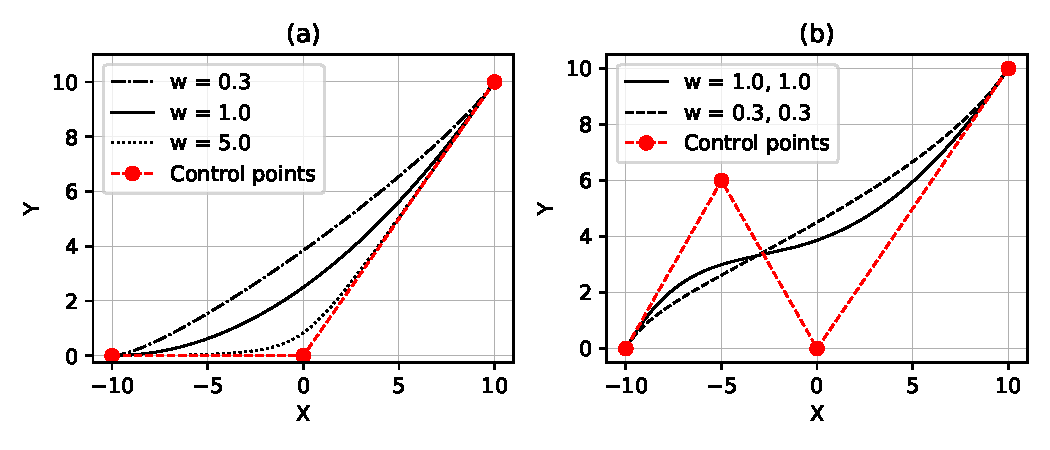
\includegraphics[width=0.8\linewidth]{../PICS/nurbs.pdf}
  \caption{NURBS curves generated from three control points with quadratic 
  degree ($p=2$) and different weights.}
  \label{fig:nurbs}
  \end{center}
\end{figure}
Figure ~\ref{fig:nurbs} illustrates how varying the weight of the middle control 
  point affects the curve: a lower weight ($w=0.2$) pulls the curve away 
  from the point, uniform weight ($w=1.0$) yields the standard quadratic B-spline, 
  and a higher weight ($w=5.0$) attracts the curve toward the control point. 
  Red markers indicate the control points used for all curves.
\begin{table}[H]
\centering
\begin{tabular}{l c c c}
\hline
AF & $y$ & $x_{\kappa' = 0}$ & $\kappa_{\text{max}}$\\
\hline
\texttt{Tanh}~\ref{app:tanh} & $\frac{e^{x} - e^{-x}}{e^{x} - e^{-x}}$ & 0.9196 & 0.5073\\
\texttt{Sigmoid}~\ref{app:sigmoid} & $\frac{1}{1 + e^{-x}}$ & 1.3819 & 0.0924\\
\texttt{Softplus}~\ref{app:softplus} & $\ln{({1 + e^{x}})}$ & -0.5 & 0.1913\\
\texttt{ELU}~\ref{app:elu} & $
\begin{cases}
  x & \text{if } x \geq 0, \\
  \alpha (e^x - 1) & \text{if } x < 0
\end{cases}$ & $-\frac{1}{2} \ln(2 \alpha^2)$ & $\frac{2}{3\sqrt3}$\\
\texttt{SiLU}~\ref{app:silu} & $x \cdot \frac{1}{1 + e^{-x}}$ & -0.3768 & 0.4037 \\
\texttt{GELU}~\ref{app:gelu} & $x \phi(x)$ & -0.4773 & 1.3579\\
\texttt{ReLU} & $
\begin{cases}
x, & \text{if } x > 0, \\
0, & \text{if } x \le 0.
\end{cases}$ & undefined & undefined\\
\texttt{Leaky-ReLU} & $
\begin{cases}
x, & \text{if } x > 0, \\
\alpha x, & \text{if } x \le 0.
\end{cases}$ & undefined & undefined\\
\texttt{LeLU}~\ref{app:LeLU} & $
\begin{cases}
x, & \text{if } x > 0, \\
e^{(1 - \beta)x} - 1 + \beta x, & \text{if } x \le 0.
\end{cases}$ & $- \frac{\sqrt{2}}{2}\ln2$ & 0.3924\\
\texttt{Mish}~\ref{app:mish} & $x \cdot \tanh\!\left(\ln(1 + e^{x})\right)$ & -0.4271 & 0.5900\\
\hline
\end{tabular}
\caption{AF with their peak curvature values and the input positions at which these maxima occur.}
\label{tab:AF}
\end{table}

\begin{figure}[H]
  \begin{center}
    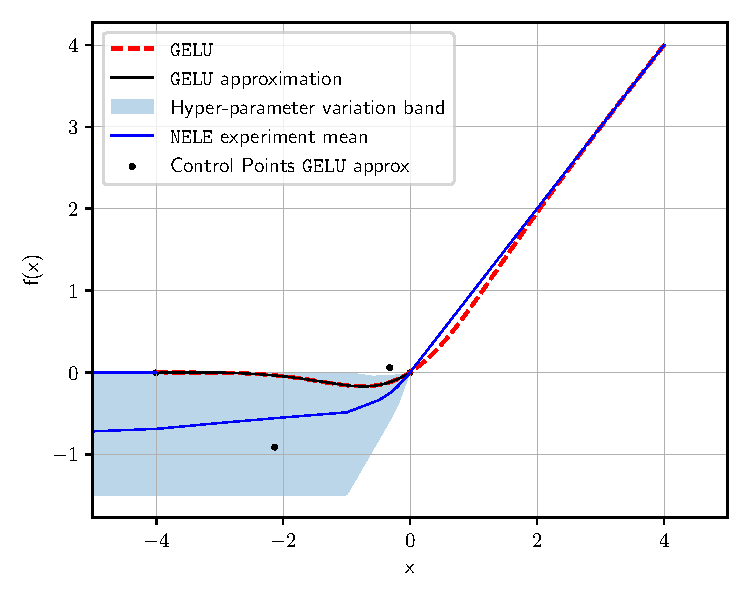
\includegraphics[width=0.85\linewidth]{../PICS/Approx_gelu.pdf}
  \caption{GELU approximated for $x \leq 0$ using cubic NURBS with 3 control points and optimized weights.
  NURBS curve used for MNIST study is also shown for comparison. }
  \label{fig:nurbsregen}
  \end{center}
\end{figure}
\texttt{NELE} can be constructed in a piecewise manner. For $x > 0$, a linear segment is used, 
while for $x \leq 0$, a cubic NURBS curve with three control points and optimized weights is employed.
This design choice can mimic the behavior of \texttt{ReLU} in the positive domain, and \texttt{GELU} in the negative domain.
Other configurations like using NURBS for both positive and negative domains or even limiting the negative space are possible. 
The key advantage of cubic NURBS lies in the ability to construct curves with inflection points. 
Control points and weights used can also be learnable paramters, but this adds additional complexity to the training process.
To approximate a target curve with \texttt{NELE}, an optimization problem is formulated to minimize the mean squared error (MSE) between the target function and the NURBS representation.
Optimization algorithm L-BFGS-B \cite{scipy_optimize_minimize} is used to efficiently navigate the parameter space, 
producing a smooth curve that closely follows the desired shape. The parametric values for different AF
are given in Appendix~\ref{app:nurbsparams}.

\section{Experiments with \texttt{NELE}}
Following the construction process outlined in~\ref{fig:nurbsregen}, \texttt{NELE} is benchmarked against \texttt{tanh}, \texttt{sigmoid}, \texttt{softplus}, \texttt{ELU}, \texttt{SiLU}, \texttt{GELU}, \texttt{ReLU}, \texttt{Leaky ReLU}, \texttt{LeLU} \cite{BIGARELLA2026122739} and \texttt{Mish}. The following datasets are used: 
(i)  Non-linear synthetic data (NLSD), (ii) MNIST \cite{lecun1998mnist}, (ii) MNIST encoder, (iv) CIFAR-10 \cite{hope2017learning}
 and (v) CIFAR-100 \cite{krizhevsky2009cifar}.

\subsection{Non-linear synthetic data}
The neural network used for curve fitting consists of a fully connected feedforward 
architecture with a single hidden layer of 64 neurons. 
The hidden layer employs the various AF, while the output layer is linear. 
In schematic form, the network can be represented as:
\[
x \;\xrightarrow{\text{Linear } (\text{input\_dim} \to 64)}\;
\text{AF} \;\xrightarrow{\text{Linear } (64 \to 1)}\; y
\]
The model was trained with Mean-Squared-Error (MSE) loss \cite{BickelDoksum2015MathStats}.
MSE provides a smooth, differentiable penalty for prediction errors, 
emphasizes larger deviations, and produces outputs that closely follow 
the target curve \cite{Bishop2006PRML}, which is important for subsequent smoothness analysis.
To evaluate the performance of different AF for function approximation, 
a series of synthetic datasets representing diverse nonlinear relationships is generated. 
Specifically, the target outputs $y$ were constructed as follows:
\begin{align*}
y_1 &= \sin(x) + \epsilon\tag{a} \\
y_2 &= \sin(x) + 0.5 \cdot \sin(3x) + \epsilon\tag{b} \\
y_3 &= e^{-0.5 x} + \epsilon\tag{c} \\
y_4 &= \tanh(x) + \epsilon\tag{d} \\
y_5 &= x^2 +  \epsilon\tag{e} \\
y_6 &= \frac{x^3}{e^{x} - 1 + 10^{-6}} + \epsilon\tag{f}
\end{align*}

where $\epsilon \sim \mathcal{N}(0,1)$ denotes Gaussian noise added to simulate measurement 
or environmental variability. The chosen functions span a range of behaviors, 
including oscillatory patterns, exponential decay, saturating nonlinearities 
and polynomial growth, thereby providing a comprehensive testbed for assessing the 
generalization capability of different neural network architectures.
Each dataset was used to train feedforward neural networks with various AF. 
The networks were evaluated based on their ability to fit the underlying 
function while mitigating overfitting to noise ($\epsilon = 0.2$). Each model was trained for 
a maximum of 300 epochs with a learning rate ($10^{-2}$, $10^{-3}$, $10^{-4}$) and parameter initialisation 
optimised to give the lowest training loss.
The studies were repeated across 7 runs
and the median training loss across these runs is shown in 
Figure~\ref{fig:Lossplottrend}.
Preliminary results indicate that AF with smooth, bounded characteristics 
(e.g., \texttt{Tanh}, \texttt{Sigmoid}) excel in capturing oscillatory 
and saturating patterns.
These findings highlight the importance of matching AF properties 
to the underlying target function characteristics in curve-fitting tasks.
Given a set of discrete points $\{(x_i, y_i)\}_{i=1}^N$ representing a curve, 
smoothness was quantified using curvature based criteria:
For a parametric curve $(x(t), y(t))$, the curvature at a point is defined as
\begin{equation}
\kappa(t) = \frac{|x'(t)y''(t) - y'(t)x''(t)|}{\left( x'(t)^2 + y'(t)^2 \right)^{3/2}}
\end{equation}

The total curvature is approximated for discrete points using finite differences:
\begin{equation}
K_\text{total} = \sum_{i=1}^{N} \kappa_i
\end{equation}
\begin{figure}[H]
    \centering
    % Row 1
    \begin{subfigure}{0.32\textwidth}
        \centering
        \includegraphics[width=\linewidth]{../PICS/NLSD/exp/curve_fitting.pdf}
        \caption{Exponential + Noise}
    \end{subfigure}
    \hfill
    \begin{subfigure}{0.32\textwidth}
        \centering
        \includegraphics[width=\linewidth]{../PICS/NLSD/hyp/curve_fitting.pdf}
        \caption{Hyperbola + Noise}
    \end{subfigure}
    \hfill
    \begin{subfigure}{0.32\textwidth}
        \centering
        \includegraphics[width=\linewidth]{../PICS/NLSD/quad/curve_fitting.pdf}
        \caption{Quadratic + Noise}
    \end{subfigure}

    \vspace{0.5cm}

    % Row 2
    \begin{subfigure}{0.32\textwidth}
        \centering
        \includegraphics[width=\linewidth]{../PICS/NLSD/sine/curve_fitting.pdf}
        \caption{Sinusoidal + Noise}
    \end{subfigure}
    \hfill
    \begin{subfigure}{0.32\textwidth}
        \centering
        \includegraphics[width=\linewidth]{../PICS/NLSD/trig/curve_fitting.pdf}
        \caption{Trigonometric + Noise}
    \end{subfigure}
    \hfill
    \begin{subfigure}{0.32\textwidth}
        \centering
        \includegraphics[width=\linewidth]{../PICS/NLSD/exppoly/curve_fitting.pdf}
        \caption{Polynomial + Noise}
    \end{subfigure}

    \caption{Curve fitting results for different target functions 
    using the proposed neural network, illustrating the network's 
    ability to approximate diverse nonlinear patterns.}
    \label{fig:curvefittingtrend}
\end{figure}

\begin{table}[h!]
\centering
\begin{tabular}{|l|llllll|}
\hline
\bfseries AF & \multicolumn{6}{c|}{\bfseries $K_\text{total}$} \\
\cline{2-7}
 & (a) & (b) & (c) & (d) & (e) & (f) \\
\hline
\texttt{Tanh} & 46.72 & 39.51 & 41.47 & 73.0 & 155.65 & 35.13 \\ 
\texttt{Sigmoid} & 26.86 & 31.5 & 44.09 & 63.14 & 68.48 & 27.32 \\ 
\texttt{Softplus} & 31.96 & 34.94 & 39.45 & 55.88 & 57.04 & 23.04 \\ 
\texttt{ELU} & 45.33 & 33.36 & 39.77 & 57.36 & 61.63 & 23.44 \\ 
\texttt{SiLU} & 46.02 & 32.34 & 39.51 & 57.38 & 64.14 & 30.44 \\ 
\texttt{GELU} & 77.24 & 34.76 & 41.84 & 61.93 & 107.0 & 50.47 \\ 
\texttt{ReLU} & 107.69 & 55.85 & 51.58 & 75.75 & 79.89 & 51.41 \\ 
\texttt{Leaky-ReLU} & 96.3 & 52.63 & 47.37 & 66.68 & 79.93 & 34.55 \\ 
\texttt{LeLU} & 27.58 & 31.24 & 39.82 & 69.49 & 111.18 & 19.86 \\ 
\texttt{Mish} & 60.13 & 34.1 & 43.28 & 59.05 & 60.72 & 28.71 \\ 
\texttt{NELE} & 44.02 & 38.33 & 41.4 & 61.62 & 114.7 & 30.81 \\ 
\hline
\end{tabular}
\caption{Comparison of smoothness metrics for different activation functions and \texttt{NELE} tuned for lowest training loss. 
The table reports total curvature ($K_\text{total}$) for each AF. 
Lower values indicate smoother behavior. The lowest value in each column 
is highlighted in \textbf{bold}, indicating the smoothest curve.}
\label{tab:smooth}
\end{table}
Among the AF evaluated, the proposed \texttt{NELE} activation 
consistently demonstrates comparable and sometimes superior performance across all benchmark functions. 
Quantitatively, networks employing \texttt{NELE} achieve lower training loss and smaller 
standard deviation of curve-fitting errors relative to alternative activations, 
indicating both improved accuracy and enhanced reliability.

\begin{figure}[H]
    \centering

    % Row 1
    \begin{subfigure}{0.32\textwidth}
        \centering
        \includegraphics[width=\linewidth]{../PICS/NLSD/exp/Loss_Bar_Chart_with_Error_Bars.pdf}
        \caption{Exponential + Noise}
    \end{subfigure}
    \hfill
    \begin{subfigure}{0.32\textwidth}
        \centering
        \includegraphics[width=\linewidth]{../PICS/NLSD/hyp/Loss_Bar_Chart_with_Error_Bars.pdf}
        \caption{Hyperbola + Noise}
    \end{subfigure}
    \hfill
    \begin{subfigure}{0.32\textwidth}
        \centering
        \includegraphics[width=\linewidth]{../PICS/NLSD/quad/Loss_Bar_Chart_with_Error_Bars.pdf}
        \caption{Quadratic + Noise}
    \end{subfigure}

    \vspace{0.5cm}

    % Row 2
    \begin{subfigure}{0.32\textwidth}
        \centering
        \includegraphics[width=\linewidth]{../PICS/NLSD/sine/Loss_Bar_Chart_with_Error_Bars.pdf}
        \caption{Sinusoidal + Noise}
    \end{subfigure}
    \hfill
    \begin{subfigure}{0.32\textwidth}
        \centering
        \includegraphics[width=\linewidth]{../PICS/NLSD/trig/Loss_Bar_Chart_with_Error_Bars.pdf}
        \caption{Trigonometric + Noise}
    \end{subfigure}
    \hfill
    \begin{subfigure}{0.32\textwidth}
        \centering
        \includegraphics[width=\linewidth]{../PICS/NLSD/exppoly/Loss_Bar_Chart_with_Error_Bars.pdf}
        \caption{Polynomial + Noise}
    \end{subfigure}

    \caption{Standard deviation of prediction errors for different target functions, illustrating 
    the variability in the neural network's curve fitting performance. Despite \texttt{LeLU} 
    reaching a lower training loss for the sinusoidal function, 
    the corresponding fit lacks smoothness.}
    \label{fig:standarddevtrend}
\end{figure}
Following the recommended procedure for \texttt{LELU}, the neural network should 
be trained via backpropagation to minimize the mean absolute error (MAE) 
between the predicted values and the true function at the training points, 
followed by computation of diffusion terms and application of the diffusion loss. 
In the experiments, however, only the standard MSE loss was used. 
Under these conditions, \texttt{NELE} produced  
predictions with smoothness comparable to \texttt{LeLU} and training 
loss values that were lower or similar across all benchmark functions.
\begin{figure}[H]
    \centering

    % Row 1
    \begin{subfigure}{0.32\textwidth}
        \centering
        
\includegraphics[width=\linewidth]{../PICS/NLSD/exp/training_loss.pdf}
        \caption{Exponential + Noise}
    \end{subfigure}
    \hfill
    \begin{subfigure}{0.32\textwidth}
        \centering
        
\includegraphics[width=\linewidth]{../PICS/NLSD/hyp/training_loss.pdf}
        \caption{Hyperbola + Noise}
    \end{subfigure}
    \hfill
    \begin{subfigure}{0.32\textwidth}
        \centering
        
\includegraphics[width=\linewidth]{../PICS/NLSD/quad/training_loss.pdf}
        \caption{Quadratic + Noise}
    \end{subfigure}

    \vspace{0.5cm}

    % Row 2
    \begin{subfigure}{0.32\textwidth}
        \centering
        
\includegraphics[width=\linewidth]{../PICS/NLSD/sine/training_loss.pdf}
        \caption{Sinusoidal + Noise}
    \end{subfigure}
    \hfill
    \begin{subfigure}{0.32\textwidth}
        \centering
        
\includegraphics[width=\linewidth]{../PICS/NLSD/trig/training_loss.pdf}
        \caption{Trigonometric + Noise}
    \end{subfigure}
    \hfill
    \begin{subfigure}{0.32\textwidth}
        \centering
        
\includegraphics[width=\linewidth]{../PICS/NLSD/exppoly/training_loss.pdf}
        \caption{Polynomial + Noise}
    \end{subfigure}

    \caption{Training loss curves for the neural network across different target functions, 
    showing the convergence behavior and learning dynamics for each 
    functional form and AF.}
    \label{fig:Lossplottrend}
\end{figure}

\subsection{MNIST}
The performance of various activation functions was evaluated by 
replicating the experimental setup of \cite{hendrycks2023gaussianerrorlinearunits}.
Fully connected neural networks with eight hidden layers of 128 neurons each were trained
using AF listed in Table~\ref{tab:smooth}. 
All networks were trained using the Adam optimizer with cross-entropy loss \cite{mao2023crossentropylossfunctionstheoretical} and
learning rates of $10^{-3}$, $10^{-4}$, and $10^{-5}$. Validation used $5,000$ samples 
to select the best model. In total, seven runs were performed for 75 epochs on the complete 
dataset with the optimized hyperparameters and their median values are used for comparison.
\texttt{NELE} was stopped early at epoch 50 as it showed comparable convergence to other AF.
Figure~\ref{fig:mnistloss} shows how each AF influences convergence speed and final loss.
\begin{figure}[H]
  \begin{center}
    
\includegraphics[width=1.0\linewidth]{../PICS/MNIST/training_loss.pdf}
  \caption{Training and test accuracy trends for MNIST over epochs using different AF. Differences in the test accuracy curves reflect 
  the varying generalization performance of each AF.\label{fig:mnistloss}}
  \end{center}
\end{figure}
\begin{figure}[H]
  \begin{center}
    \includegraphics[width=0.8\linewidth]{../PICS/MNIST/noise_study.pdf}
  \caption{Robustness results for MNIST over noise strengths using different AF.\label{fig:mnistnoise}}
  \end{center}
\end{figure}
\texttt{NELE} converged within 30 epochs with a 
learning rate (\textit{lr}) of $0.001$ and achieved the lowest test error~\ref{tab:mnisttesult}. 
The trained model was also tested
with inputs containing uniform noise Unif[-a,a] added to each example at different levels a, where
a = 3 is the greatest noise strength. 
Here, \texttt{NELE} shows good robustness with its performace matching \texttt{GELU} and exceeding
other AF.
\begin{table}[H]
  \centering
\begin{tabular}{@{}llll@{}}
  \toprule
  \makecell[l]{\textbf{AF}} &
\makecell[l]{\textbf{Training} \\ \textbf{Loss}} &
\makecell[l]{\textbf{Test error} \\ \textbf{w/o noise (\%)}} &
\makecell[l]{\textbf{Test score} \\ \textbf{w noise (\%)}} \\
\midrule
  \texttt{Tanh} & 0.0076 & 2.7 & 22.94\\
\texttt{Sigmoid} & 0.0072 & 4.45 & 16.47\\
\texttt{Softplus}& 0.004 & 2.52 & 22.37\\
\texttt{ELU}& 0.0056 & 2.44 & 21.51\\
\texttt{SiLU} & 0.0045 & 2.28 & 24.64\\
\texttt{GELU} & 0.0049 & 2.32 & 24.89\\
\texttt{ReLU} & 0.0054 & 2.32 & 23.02\\
\texttt{Leaky-ReLU}& 0.0044 & 2.35 & 21.22\\
\texttt{LeLU} & 0.0002 & 2.12 & 18.5\\
\texttt{Mish} & 0.0056 & 2.32 & 24.31\\
\texttt{NELE}& 0.0056 & \textbf{1.83} & \textbf{25.49}\\
  \bottomrule
\end{tabular}
\caption{Comparison of training loss and test error on the MNIST classification task
trained with different AF. \texttt{NELE} achieves the 
lowest test error among all activations evaluated.}\label{tab:mnisttesult}
\end{table}
\subsection{MNIST autoencoder}
The neural netowrk is a deep autoencoder from \cite{desjardins2015naturalneuralnetworks}
with Adam optimizer and a batch size of 64. A learning rate of $10^{-3}$ was used 
with Mean Squared Error loss. Figure~\ref{fig:mnistenc} shows that
with settings of \texttt{NELE} from Figure~\ref{fig:nurbsregen}, the AF
can perform quite well in tests.
\begin{figure}[H]
  \begin{center}
    
\includegraphics[width=1.0\linewidth]{../PICS/MNIST_ENC/training_loss.pdf}
  \caption{Training loss and test reconstruction error 
  trends for MNIST autoencoder over epochs using 
  different AF.\label{fig:mnistenc}}
  \end{center}
\end{figure}
\subsection{CIFAR-10}
The neural network is a 9-layer network with the architecture and training
procedure from \cite{hendrycks2023gaussianerrorlinearunits}. The tuning was done 
using learning rates of $10^{-3}$, $10^{-4}$, and $10^{-5}$ for 100 epochs.
The best model was selected based on validation accuracy using 5,000 samples.
Seven runs were performed and the median values are reported.
Figure~\ref{fig:cifar10loss} shows the training loss and test accuracy calculated every 5 epochs for CIFAR-10 over epochs using different AF.

\begin{figure}[H]
  \begin{center}
    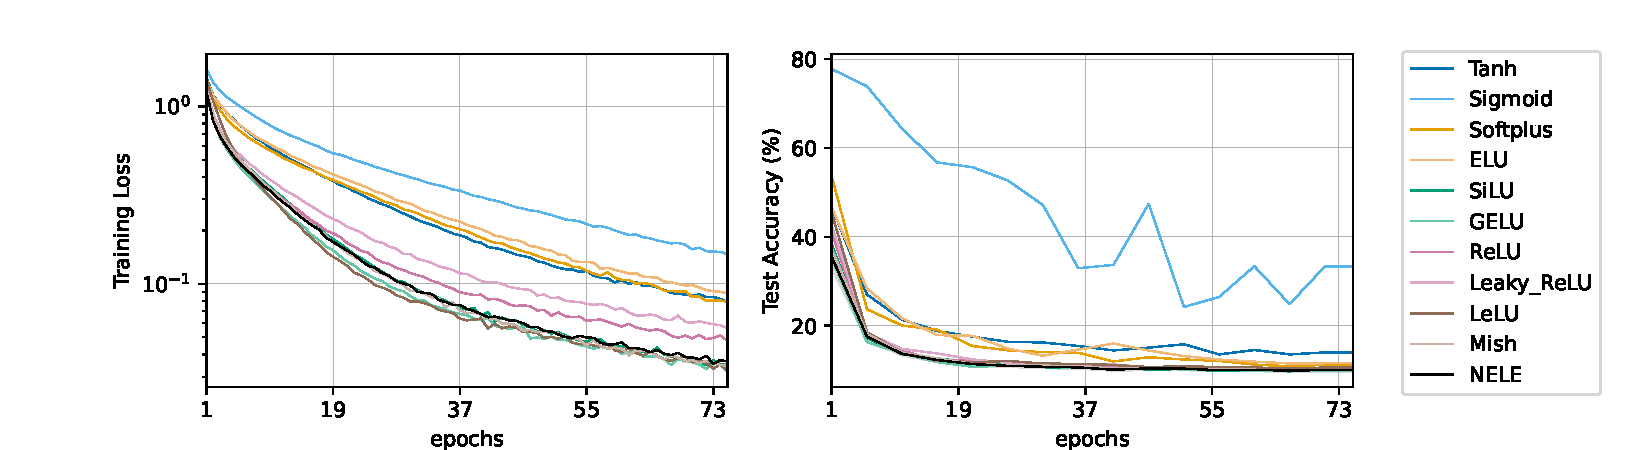
\includegraphics[width=1.0\linewidth]{../PICS/CIFAR10/training_loss.pdf}
  \caption{Training and test accuracy trends for CIFAR10 over epochs using different AF.}
  \label{fig:cifar10loss}
  \end{center}
\end{figure}
\subsection{CIFAR-100}
The model for CIFAR-100 is a wide residual neural network described in 
\cite{zagoruyko2017wideresidualnetworks} with learning rate scheduler and dropout keep
probability from
\cite{loshchilov2017sgdrstochasticgradientdescent} and batch normalization 
at the end of a residual block to stabilize exploding ELU's \cite{Shah_2016}
as implemented in \cite{hendrycks2023gaussianerrorlinearunits}. Setting from Figure~\ref{fig:nurbsregen} 
were used to obtain Median convergence
curves over seven runs as shown in Figure~\ref{fig:cifar100loss}.

\begin{figure}[H]
  \begin{center}
    
\includegraphics[width=1.0\linewidth]{../PICS/CIFAR100/training_loss.pdf}
  \caption{Training and test accuracy trends for CIFAR100 over 50 epochs using different AF.}
  \label{fig:cifar100loss}
  \end{center}
\end{figure}
\section{Conclusion}
\texttt{NELE} offers several desirable properties for functional approximation: 
smoothness, local control, geometric interpretability, and the ability to 
represent both polynomial and non-polynomial shapes using a small number of 
control points.
\appendix{}
\section{Function analysis}
\begin{figure}[H]\label{fig:afcollect}
  \begin{center}
    \includegraphics[width=1.0\linewidth]{../analysis/analysis.pdf}
  \caption{The solid lines represent the functions $y(x)$ for different activation functions. 
The points of maximum curvature, $\kappa_{\mathrm{max}}$, are indicated by markers along each curve. 
The dashed lines represent the curvature, $\kappa(x)$, as a function of $x$. 
Each color corresponds to a different activation function as shown in the legend.}
  \end{center}
\end{figure}
\newpage
\subsection{tanh}\label{app:tanh}
\begin{wrapfigure}{r}{0.45\textwidth}
    \centering
    \vspace{-10pt}
    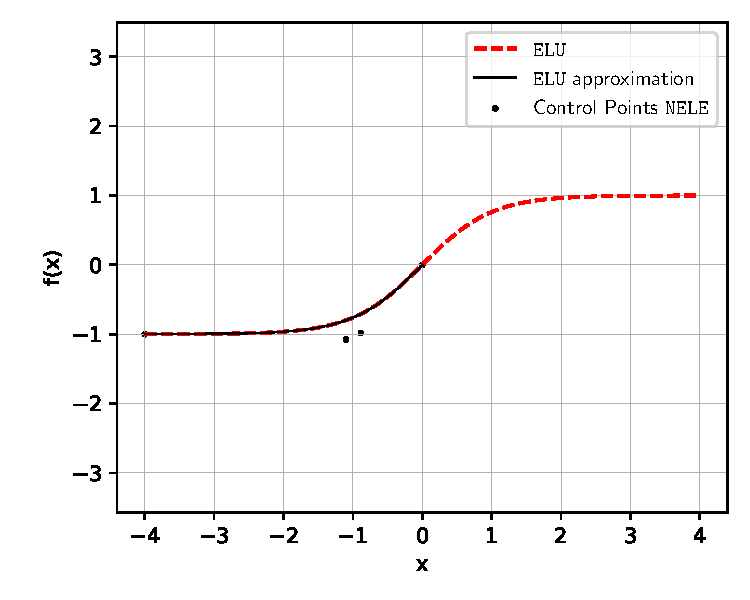
\includegraphics[width=0.35\textwidth]{../PICS/Approx_tanh.pdf} % replace with your figure
    \caption{\texttt{NELE} approximation of \texttt{tanh}}
    \vspace{-10pt}
\end{wrapfigure}
$y = \tanh{x}$\\\\
$y' = \operatorname{sech}^2(x) = 1 - y^2$\\\\
$y'' = -2\operatorname{sech}^2(x)\tanh{x} = -2y(1 - y^2)$\\\\
$\kappa = \frac{|-2\operatorname{sech}^2(x)\tanh{x}|}{(1 + (\operatorname{sech}^2(x))^2)^\frac{3}{2}}$\\\\
$\frac{d \kappa}{dx} = 0$, using chain rule 
$\frac{d \kappa}{dx} = \frac{d \kappa}{dy}\frac{dy}{dx}$\\\\
Then, $\frac{d \kappa}{dy} = 0$ or $1 - y^2 = 0$\\\\
$\frac{d}{dy}\left( \frac{2y(1 - y^2)}{(1 + (1 - y^2)^2)^{3/2}}\right)
= 3y^6 - 5y^4 - 2y^2 + 2 = 0$\\\\
Solving: $y = 0.9196$, $\kappa_{\max} = 0.5073$

\subsection{Sigmoid}\label{app:sigmoid}
\begin{wrapfigure}{r}{0.45\textwidth}
    \centering
    \vspace{-10pt}
    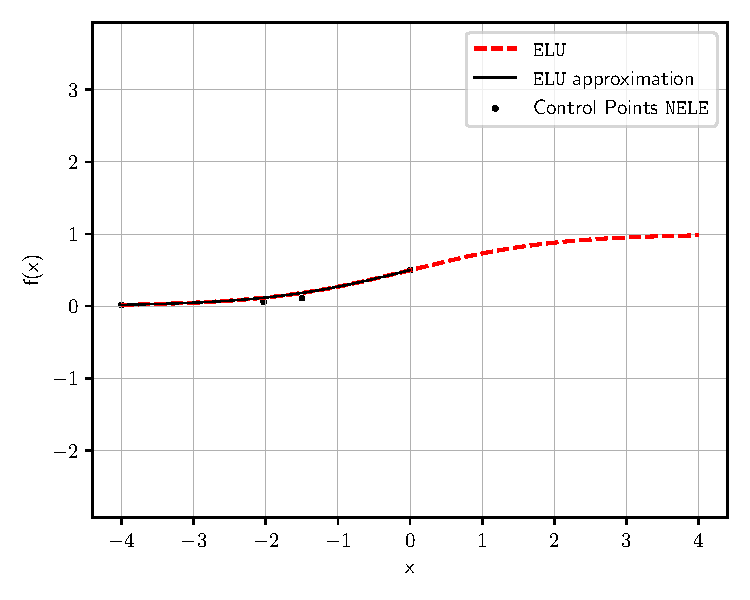
\includegraphics[width=0.35\textwidth]{../PICS/Approx_sigmoid.pdf} % replace with your figure
    \caption{\texttt{NELE} approximation of \texttt{sigmoid}}
    \vspace{-10pt}
\end{wrapfigure}
$y = \frac{1}{1 + e^{-x}}$\\\\
$y' = \frac{-e^{-x}}{(1 + e^{-x})^2}$\\\\
$y'' = \frac{e^{-x}(1 - e^{-x})}{(1 + e^{-x})^3}$\\\\
$\kappa = \frac{\frac{e^{-x}(1 - e^{-x})}{(1 + e^{-x})^3}}{(1 + ( \frac{-e^{-x}}{(1 + e^{-x})^2})^2)^\frac{3}{2}}$\\\\
Solving this equation leads to a transcendental condition, 
which has no simple closed-form solution, so the 
locations of maximum curvature must be obtained numerically.

\subsection{Softplus}\label{app:softplus}
\begin{wrapfigure}{r}{0.45\textwidth}
    \centering
    \vspace{-10pt}
    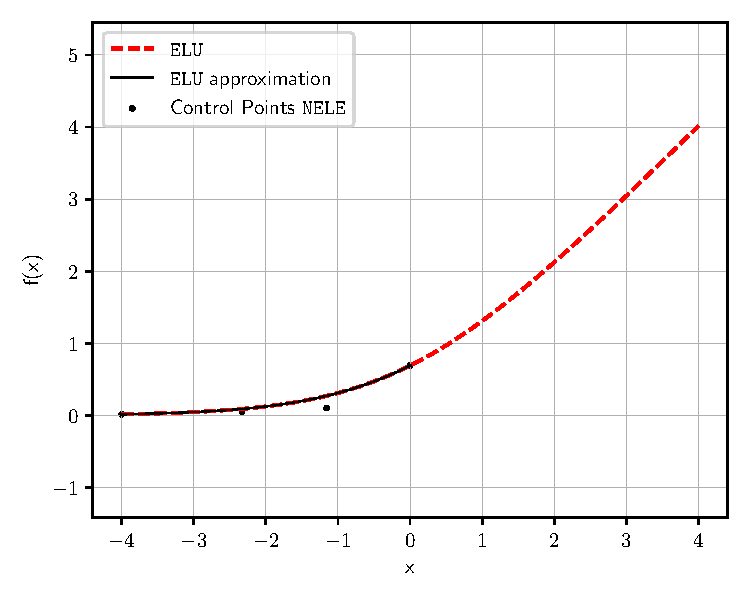
\includegraphics[width=0.35\textwidth]{../PICS/Approx_softplus.pdf} % replace with your figure
    \caption{\texttt{NELE} approximation of \texttt{softplus}}
    \vspace{-10pt}
\end{wrapfigure}
$y = \ln{({1 + e^{x}})}$\\\\
$y' = \frac{e^x}{1 + e^x}$\\\\
$y'' = \frac{e^{x}}{(1 + e^{x})^2}$\\\\
$\kappa = \frac{\frac{e^{x}}{(1 + e^{x})^2}}{(1 + (\frac{e^x}{1 + e^x})^2)^\frac{3}{2}}$\\\\
Let $s = \frac{e^x}{1 + e^x}$, $\kappa = \frac{s(1 - s)}{(1 + s^2)^\frac{3}{2}}$\\\\
$\frac{d\kappa}{dx} = 0$, $\frac{d}{dx}\bigg(\frac{s(1 - s)}{(1 + s^2)^\frac{3}{2}}\bigg) = 0$\\\\
Solving $s = -1, 0.38197, 2.6180$\\\\
Substituting, $x = -0.5$, $\kappa_{\text{max}} = 0.1913$

\subsection{ELU}\label{app:elu}
\begin{wrapfigure}{r}{0.45\textwidth}
    \centering
    \vspace{-10pt}
    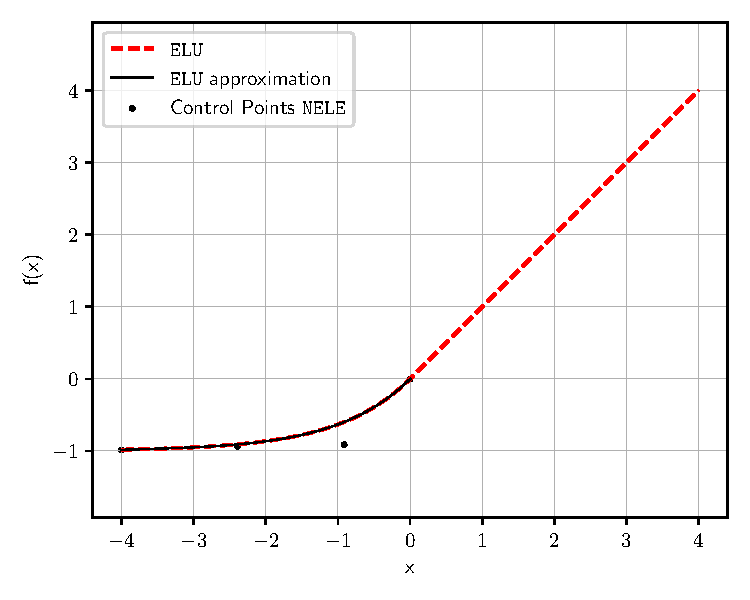
\includegraphics[width=0.35\textwidth]{../PICS/Approx_elu.pdf} % replace with your figure
    \caption{\texttt{NELE} approximation of \texttt{ELU}}
    \vspace{-10pt}
\end{wrapfigure}
$y = \begin{cases}
  x & \text{if } x \geq 0, \\
  \alpha (e^x - 1) & \text{if } x < 0
\end{cases}$
\\\\
$y' = \begin{cases}
  1 & \text{if } x \geq 0, \\
  \alpha e^x & \text{if } x < 0
\end{cases}$
and 
$y'' = \begin{cases}
  0 & \text{if } x \geq 0, \\
  \alpha e^x & \text{if } x < 0
\end{cases}$
\\\\
$\kappa = \begin{cases}
  0 & \text{if } x \geq 0, \\
  \frac{\alpha e^x}{(1 + \alpha^2 e^{2x})^\frac{3}{2}}  & \text{if } x < 0
\end{cases}$
\\\\
$\frac{d \kappa}{dx} = 0$
\\\\
$\frac{d}{dx} \left( \frac{\alpha e^x}{(1 + \alpha^2 e^{2x})^{3/2}} \right)
= \frac{\alpha e^x \left( 1 - 2 \alpha^2 e^{2x} \right)}{(1 + \alpha^2 e^{2x})^{5/2}} = 0$
\\\\
$\alpha e^x \left( 1 - 2 \alpha^2 e^{2x} \right) = 0$
\\\\
$e^x = 0 \quad \text{has no solution}$, therefore, $x = -\frac{1}{2} \ln(2 \alpha^2)$
\\\\
Substituting back, $\kappa_{\text{max}} = \frac{2}{3\sqrt3}$

\subsection{SiLU}\label{app:silu}
\begin{wrapfigure}{r}{0.45\textwidth}
    \centering
    \vspace{-10pt}
    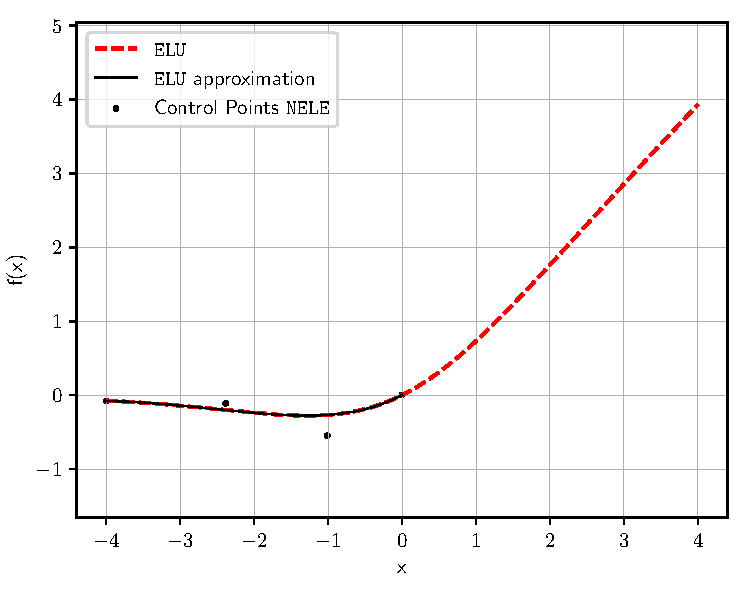
\includegraphics[width=0.35\textwidth]{../PICS/Approx_silu.pdf} % replace with your figure
    \caption{\texttt{NELE} approximation of \texttt{SiLU}}
    \vspace{-10pt}
\end{wrapfigure}
$y = \frac{x}{1 + e^{-x}}$
\\\\
$y' = \frac{1 + e^{-x} + xe^{-x}}{(1 + e^{-x})^2}$
\\\\
$y'' = \frac{e^{-x}(2 - x) + e^{-2x}(x+2)}{(1 + e^{-x})^3}$
\\\\
$\kappa = \frac{\frac{e^{-x}(2 - x) + e^{-2x}(x+2)}{(1 + e^{-x})^3}}{(1 + (\frac{1 + e^{-x} + xe^{-x}}{(1 + e^{-x})^2})^2)^\frac{3}{2}}
= \frac{(1 + e^{-x})^2(e^{-x}(2 - x) + e^{-2x}(x+2))}{[(1 + e^{-x})^4 + (1 + e^{-x} + xe^{-x})^2]^\frac{3}{2}}$
\\\\
$\frac{d \kappa}{dx} = 0$
\\\\
$\frac{d}{dx}\biggr(\frac{(1 + e^{-x})^2(e^{-x}(2 - x) + e^{-2x}(x+2))}{[(1 + e^{-x})^4 + (1 + e^{-x} + xe^{-x})^2]^\frac{3}{2}}\biggr) = 0$
\\\\
Using quotient rule and consider the first term in the numerator after differentiation :
$[e^{-x}(x-3)-e^{-2x}(2x+3)](1+e^{-x})^2$. This leads to a nonlinear 
transcendental equation. Since, they do not simplify into algebraic 
forms that allow symbolic isolation of x, an exact analytical solution for the location of 
maximum curvature is not possible and numerical or graphical methods must be used.

\subsection{GELU}\label{app:gelu}
$y = x \phi(x) \approx 0.5x(1 + \tanh [\sqrt{2 / \pi}(x + 0.44715 x^3)])$
\\
Let $k = \sqrt{\frac{2}{\pi}}$, $a = 0.441715$ and $u(x) = k(x + ax^3)$\\
$y' = 0.5(1 + \tanh{u}) + 0.5ax\operatorname{sech}^2(u)(1 + 3ax^2)$\\
$y'' = 0.5a(1 + 3ax^2)\operatorname{sech}^2(u) + 0.5x[-2\operatorname{sech}^2(u)\tanh{u}(a(1 + 3ax^2))^2 + 6kax\operatorname{sech}^2(u)]$

\subsection{Mish}\label{app:mish}
\begin{wrapfigure}{r}{0.45\textwidth}
    \centering
    \vspace{-10pt}
    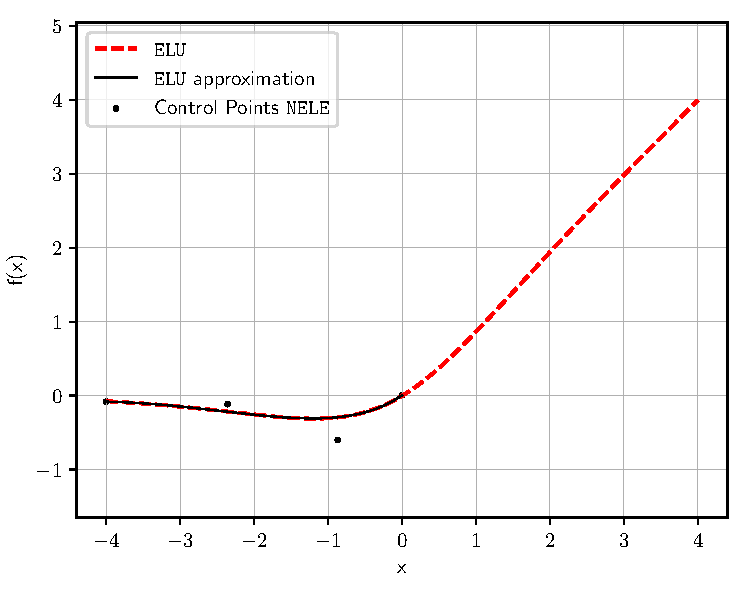
\includegraphics[width=0.35\textwidth]{../PICS/Approx_mish.pdf} % replace with your figure
    \caption{\texttt{NELE} approximation of \texttt{Mish}}
    \vspace{-10pt}
\end{wrapfigure}
$y = x \cdot \tanh\!\left(\ln(1 + e^{x})\right)$\\\\
$y' = \tanh{(\ln{(1 + e^x)})} + \frac{xe^x}{1 + e^x}\operatorname{sech}^2(\ln{(1 + e^x)})$\\\\
$y'' = \frac{e^x}{1 + e^x}\operatorname{sech}^2(\ln{(1 + e^x)})
+ \frac{\operatorname{sech}^2(\ln{(1 + e^x)})}{1+e^{-x}} 
+ \frac{xe^{-x}}{(1 + e^{-x})^2} \operatorname{sech}^2(\ln{(1 + e^x)}) \\\\
+ \frac{-2x}{(1 + e^{-x})^2} \operatorname{sech}^2(\ln{(1 + e^x)} \tanh{\ln{(1 + e^x)}}$
\\\\\\\\
\subsection{LeLU}\label{app:LeLU}
\begin{wrapfigure}{r}{0.45\textwidth}
    \centering
    \vspace{-10pt}
    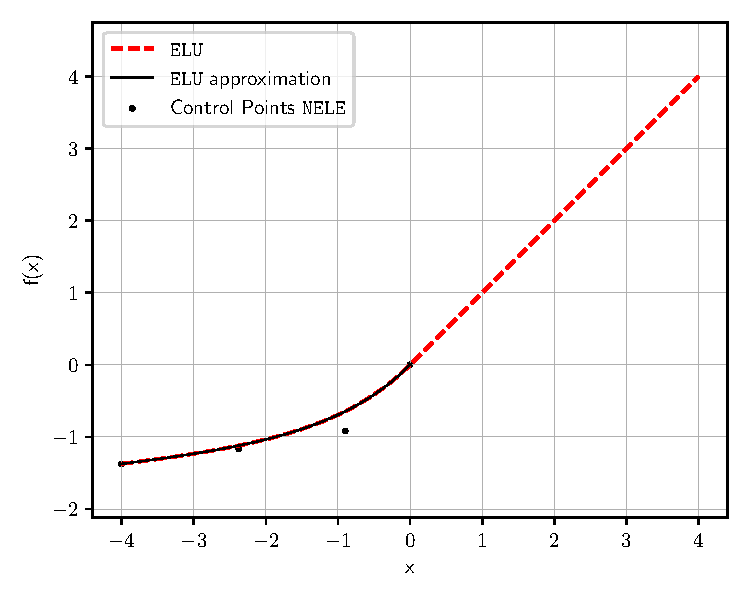
\includegraphics[width=0.35\textwidth]{../PICS/Approx_lelu.pdf} % replace with your figure
    \caption{\texttt{NELE} approximation of \texttt{LeLU}}
    \vspace{-10pt}
\end{wrapfigure}
$y = e^{(1 - \beta)x} + 1 - \beta x$\\\\
$y' = (1 - \beta)e^{(1 - \beta)x} - \beta$\\\\
$y'' = (1 - \beta)^2e^{(1 - \beta)x}$\\\\
Let $1 - \beta = a$, $e^{(1 - \beta)x} = e^{ax} = b$\\\\
$\kappa = \frac{a^2b}{(1 + a^2b^{2})^\frac{3}{2}}$\\\\
$\frac{d \kappa}{dx} = 0$\\\\
Solving, $\beta = 1 \pm \sqrt{\frac{1}{2}}, 1$, Substituting $x = 0, \pm \frac{\sqrt{2}}{2}\ln2$

\section{Curve approximation with \texttt{NELE}\label{app:nurbsparams}}
\begin{table}[H]
  \centering
  \resizebox{\textwidth}{!}{
\begin{tabular}{@{}llllllllllll@{}}
  \toprule
  \makecell[l]{\textbf{AF}} &
\makecell[c]{$p_0$} &
\makecell[c]{$p_1$} &
\makecell[c]{$p_2$} &
\makecell[c]{$p_3$} &
\makecell[c]{$w$} \\
\midrule
\texttt{Tanh} & [-3.9999, -1.0002] &    [-0.8835, -0.9828] &    [-1.0991, -1.0776] &    [0.0001, -0.001] &    [1.9424 , 0.8308 , 0.2533 , 0.2086]\\
\texttt{Sigmoid} & [-4.0, 0.0175] &    [-2.0302, 0.0589] &    [-1.4984, 0.1117] &    [0.0, 0.5012] &    [1.3098 , 0.8864 , 0.7195 , 0.8085]\\
\texttt{Softplus} & [-4.0, 0.0172] &    [-2.3319, 0.056] &    [-1.1569, 0.1045] &    [-0.0, 0.6942] &    [1.2328 , 0.9855 , 0.8082 , 0.7013]\\
\texttt{ELU} & [-3.9997, -0.9844] &    [-2.394, -0.9351] &    [-0.9134, -0.9117] &    [0.0006, -0.0009] &    [1.2268 , 1.0172 , 0.7904 , 0.5399]\\
\texttt{SiLU} & [-4.0002, -0.0782] &    [-2.3832, -0.1116] &    [-1.0106, -0.5469] &    [-0.0, 0.0033] &    [1.2261 , 1.0118 , 0.806 , 0.6113]\\
\texttt{LeLU} & [-4.0004, -1.3731] &    [-2.375, -1.1663] &    [-0.8985, -0.9166] &    [-0.0006, 0.002] &    [1.235 , 1.0147 , 0.7755 , 0.5242]\\
\texttt{Mish} & [-4.0003, -0.079] &    [-2.3577, -0.113] &    [-0.8681, -0.5979] &    [-0.0005, 0.0081] &    [1.2754 , 1.0368 , 0.7791 , 0.5086]\\
\texttt{GELU} & [-4.0, 0.0] &    [-0.3213, 0.0586] &    [-2.1341, -0.9138] &    [0.0, 0.0] &    [1.9807 , 0.7178 , 0.1238 , 0.1981]\\
\bottomrule
\end{tabular}}
\caption{Control point coordinates and their respective weights for approximation on the negative space of AF using \texttt{NELE}}\label{tab:curveapprox}
\end{table}
\bibliographystyle{plain}
\bibliography{NELE}
\end{document}